\chapter{Bibliographies}
\label{ch:bibliographies}

In this chapter, a \emph{very} rough explanation on how bibliographies and their implementation work in \LaTeX\ will be given. This is not a comprehensive guide, but rather a quick overview, followed by how to set up a bibliography with this template.

\section{How Bibliographies Work in \LaTeX}
\label{sec:bib-overview}

In \LaTeX, BibTeX is often used to describe various distinct aspects, which can lead to confusion. Some reference BibTeX as the program that \LaTeX\ uses to compile the bibliography, while others refer to compilation of the file. Then there's the integration of the backend that is used to compile; \texttt{bibtex} and \texttt{biber}, and what those represent.

To start, there are two main distinctions in the bibliography process: the \emph{external programs} that process bibliography information, and roughly act as the middle-man between your \file{.bib} file and the \LaTeX\ document, and the \LaTeX\ \emph{packages} that you import into your compilation to handle the formatting of your citations and bibliography. Here is a simple view of the process:

\begin{figure}[htbp]
    \centering
    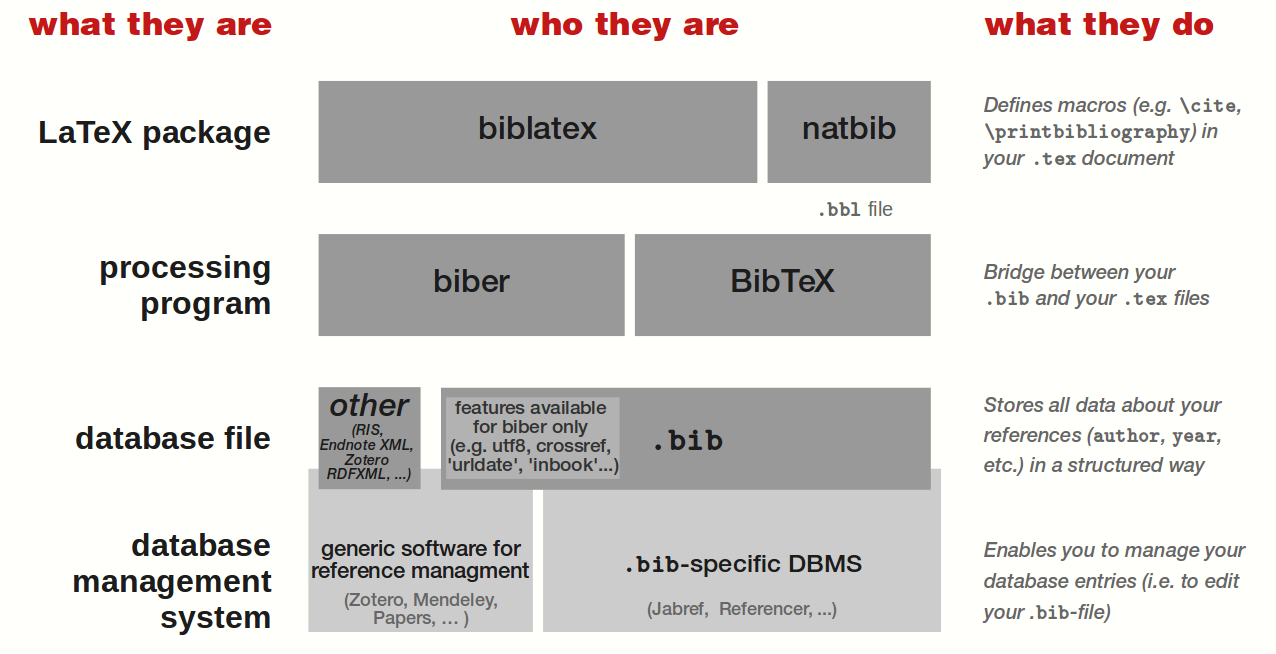
\includegraphics[width=0.8\textwidth]{citations_overview.png}
    \caption{Bibliography Process Overview in \LaTeX}
    \label{fig:bibliography-process}
\end{figure}

At the highest level, there are two main front-end \LaTeX\ packages that users interact with to handle citations, references, and bibliographies. These are \texttt{natbib} and \texttt{biblatex}. \texttt{natbib} is an older package, and although still maintained, may not be further developed. Despite this, it is still widely used, and very reliable in nature.
\texttt{biblatex} is a newer package that is more flexible and can handle more complex bibliography styles, and happens to be actively developed alongside the \texttt{biber} processing program (backend, more on this below). The humanities fields tend to use \texttt{biblatex} as many predefined styles are available (e.g., APA, MLA, Chicago). Science fields tend to go either way depending on the publishing journal's requirements and specific functionalities needed.

The backend or processing programs are the bridge between the \LaTeX\ document and the bibliography file. The two main programs are \texttt{bibtex} and \texttt{biber}. \texttt{bibtex} interfaces with specific \file{.bst} files, which are postfix language files that define the formatting of the bibliography. In the case of many major publication journals (especially in astronomy), the submission of manuscripts require the use of these \file{.bst} files, and as such, users are required to use the \texttt{natbib} \LaTeX\ package. \texttt{biber} on the other hand is a relatively newer processing program that adds further functionality to \texttt{biblatex}.

It is important to note that the \texttt{biblatex} package can make use of either the \texttt{biber} backend or the \texttt{bibtex} backend, while the \texttt{natbib} package is restricted to the \texttt{bibtex} backend. Even more importantly, results with \texttt{biblatex} can differ depending on the backend: if \texttt{bibtex} is used, it only uses it for sorting, and not for formatting content.

The takeaway is the following: if you enjoy a particular style given in a particular journal, download its \file{.bst} file and make use of the \texttt{natbib} package to compile your thesis work.

\section{Choosing a Bibliography Package}
\label{sec:bib-choosing}

The template loads the bibliography package for you, chosen with the \texttt{bibliography} class option. By default (\texttt{bibliography=none}) no bibliography package is loaded at all, so you must choose one before you can cite anything. Whichever you choose, the class adds the bibliography to the table of contents for you, as UVic requires.

\subsection{natbib}

With \texttt{bibliography=natbib}, choose a \file{.bst} style and name your \file{.bib} file at the point where the bibliography should appear. This is how the bibliography of this document is produced, using the \file{aasjournal.bst} style of the AAS journals, which is kept in the \file{extras/} folder:
\begin{lstlisting}[language=TeX]
\documentclass[bibliography=natbib]{uvicphysastro}
...
\bibliographystyle{extras/aasjournal}  % uses extras/aasjournal.bst
\bibliography{references}              % uses references.bib
\end{lstlisting}
A style file kept in \file{extras/} must be named with its folder, as above; a style file placed next to \file{thesis.tex} is named on its own (\cmd{bibliographystyle}\texttt{\{aasjournal\}}).

\texttt{natbib} provides two main citation commands: \cmd{citet} for a citation in the running text, such as \citet{Hubble1929}, and \cmd{citep} for a parenthetical citation, such as \citep{Hubble1929}.

\subsection{Numbered Citations}
\label{sec:bib-numbered}

Physics journals usually cite by number, as in ``[3, 7--9]'', rather than by author and year. With \texttt{natbib}, this needs two package options: \texttt{numbers}, and \texttt{sort\&compress}, which sorts the numbers in each citation and shortens runs such as 7, 8, 9 to 7--9. The class loads \texttt{natbib} itself, so pass the options on the first line of \file{thesis.tex}, before \cmd{documentclass} (Section~\ref{sec:packages}):
\begin{lstlisting}[language=TeX]
\PassOptionsToPackage{numbers,sort&compress}{natbib}
\documentclass[bibliography=natbib]{uvicphysastro}
\end{lstlisting}
Then cite with \cmd{citep} or \cmd{cite}. Combine this with a numbered style such as the APS style (Section~\ref{sec:bib-aps}). Do not also load the \texttt{cite} package, which older documents often use for the same purpose: \texttt{natbib} already sorts and compresses numbered citations, and warns that \texttt{cite} should not be used with it.

\subsection{biblatex}

With \texttt{bibliography=biblatex}, the class loads \texttt{biblatex} with the \texttt{biber} backend, in the style given by the \texttt{bibstyle} class option (\texttt{authoryear} by default). Name your \file{.bib} file in the preamble, and print the bibliography where it should appear:
\begin{lstlisting}[language=TeX]
\documentclass[bibliography=biblatex, bibstyle=authoryear]{uvicphysastro}
\addbibresource{references.bib}
...
\printbibliography
\end{lstlisting}
Citations use \cmd{textcite} (in the text) and \cmd{parencite} (in parentheses).

Use the citation commands of the package you chose: the \texttt{natbib} commands \cmd{citet} and \cmd{citep} are not available with \texttt{biblatex}, and \cmd{textcite} and \cmd{parencite} are not available with \texttt{natbib}. If you switch packages, replace the citation commands in your chapters as well.

\section{Journal Bibliography Styles}
\label{sec:bib-styles}

UVic does not prescribe a citation or bibliography style; follow the style guide of your field, and agree on a style with your supervisor. In astronomy, the easiest choice is usually the style of a journal you publish in, so that your thesis references look like those in your papers. With \texttt{natbib}, a journal style is a single \file{.bst} file chosen with \cmd{bibliographystyle}.

\subsection{Styles Included With the Template}

The \file{extras/} folder contains the styles of two major astronomy journals and of the American Physical Society journals (Table~\ref{tab:bib-styles}). All three are distributed under the \LaTeX\ Project Public License. The AAS and MNRAS styles are included unchanged, and are also part of every full \TeX\ installation (including Overleaf), so \cmd{bibliographystyle}\texttt{\{mnras\}} works even without the copy in \file{extras/}; the copies make sure that you use the versions this template was tested with. The APS style is a corrected copy (Section~\ref{sec:bib-aps}).

\begin{table}[htbp]
    \centering
    \caption{Journal bibliography styles included in \texttt{extras/}.}
    \label{tab:bib-styles}
    \begin{tabularx}{\linewidth}{@{}>{\raggedright\arraybackslash}X l >{\raggedright\arraybackslash}p{0.16\linewidth}@{}}
        \toprule
        Journals & Command & Version \\
        \midrule
        AAS journals (ApJ, ApJL, ApJS, AJ, PSJ) & \cmd{bibliographystyle}\texttt{\{extras/aasjournal\}} & June 2019 (AASTeX 6.3) \\
        MNRAS & \cmd{bibliographystyle}\texttt{\{extras/mnras\}} & v3.2, July 2023 \\
        APS journals (Phys.\ Rev.\ A--E, PRL, \ldots) & \cmd{bibliographystyle}\texttt{\{extras/apsrev4-2-fixed\}} & REVTeX 4.2f, corrected \\
        \bottomrule
    \end{tabularx}
\end{table}

The AAS style is deliberately the 2019 version. AAS distributes a newer \file{aasjournalv7.bst} with AASTeX~7, but it is written for the AASTeX~7 document class: used with any other class, it adds first initials to in-text citations (``E. Hubble (1929)'') and leaves stray spaces and commas in the citations and reference list.

To switch styles, change the \cmd{bibliographystyle} line and compile again; \texttt{latexmk} and Overleaf rerun BibTeX automatically.

\subsection{Physics Journals (APS)}
\label{sec:bib-aps}

The \emph{Physical Review} journals of the American Physical Society use the style \file{apsrev4-2.bst} from REVTeX, which is common in theoretical physics. It numbers the references, so use it with numbered citations (Section~\ref{sec:bib-numbered}):
\begin{lstlisting}[language=TeX]
\PassOptionsToPackage{numbers,sort&compress}{natbib}
\documentclass[bibliography=natbib]{uvicphysastro}
...
\bibliographystyle{extras/apsrev4-2-fixed}
\bibliography{references}
\end{lstlisting}
The first line passes the \texttt{numbers} and \texttt{sort\&compress} options to \texttt{natbib}: it must come before \cmd{documentclass}, because the class loads \texttt{natbib} itself.

The file is a corrected copy of \file{apsrev4-2.bst}, hence the name \file{-fixed} (the \LaTeX\ Project Public License requires a modified file to be renamed). Outside the REVTeX document class, the original style leaves a stray space before the final full stop of every reference with an arXiv number, as in ``arXiv:1807.06209 [astro-ph.CO]~.''; the copy removes that space and changes nothing else. The change is described at the top of the file.

\subsection{Other Styles}

\begin{description}
    \item[\texttt{natbib}'s own styles.] \texttt{plainnat}, \texttt{abbrvnat} and \texttt{unsrtnat} come with every \TeX\ installation and give general-purpose author--year references. Avoid \LaTeX's basic styles \texttt{plain}, \texttt{abbrv} and \texttt{unsrt} with \texttt{natbib}: they give numbered references without author names, so \cmd{citet} prints ``(author?)~[4]'' instead of the author.
    \item[Other journals.] Most journals provide a \file{.bst} file with their \LaTeX\ instructions for authors. For example, the style of \emph{Astronomy \& Astrophysics}, \file{aa.bst}, is part of the A\&A macro package available from the A\&A website (\url{https://www.aanda.org}). It is not included in this template because its licence terms do not clearly permit redistribution. Download the style, place the \file{.bst} file in \file{extras/} (or next to \file{thesis.tex}), and select it as above.
\end{description}

\section{Journal Abbreviations in \texttt{.bib} Files}
\label{sec:bib-journal-macros}

Most astronomers collect their references from the NASA Astrophysics Data System (ADS, \url{https://ui.adsabs.harvard.edu}), which exports BibTeX entries ready to paste into \file{references.bib}. For many journals, ADS writes the journal name as a \LaTeX\ macro rather than as text:
\begin{lstlisting}[language=TeX]
@ARTICLE{Planck2020,
  author = {{Planck Collaboration} and {Aghanim}, N. and {Akrami}, Y. and others},
  title = "{Planck 2018 results. VI. Cosmological parameters}",
  journal = {\aap},
  year = 2020,
  volume = {641},
  eid = {A6},
  doi = {10.1051/0004-6361/201833910},
}
\end{lstlisting}
The macro \cmd{aap} stands for \emph{Astronomy \& Astrophysics}. Journal document classes such as AASTeX and the A\&A and MNRAS classes define these macros, but standard \LaTeX\ does not: in an ordinary document, a reference to a paper in A\&A, ApJ or MNRAS stops compilation with an ``Undefined control sequence'' error.

This class defines every journal macro on ADS's list (\url{https://ui.adsabs.harvard.edu/help/actions/journal-macros}), so references exported from ADS work without any changes. Each macro prints the journal's standard abbreviation, as in the AAS and A\&A journals; Table~\ref{tab:journal-macros} shows the most common ones, and the full list is in \file{uvicphysastro.cls}. Journals that are not on ADS's list (such as \emph{Nature Astronomy} or \emph{JATIS}) are exported with their name written out in full, so they need no macro. ADS also writes the symbols $\lesssim$ and $\gtrsim$ in paper titles as the macros \cmd{lessequivlnt} and \cmd{greaterequivlnt}, which the class defines as well.

\begin{table}[htbp]
    \centering
    \caption[Common journal macros used in ADS BibTeX entries]{Common journal macros used in ADS BibTeX entries, and what they print.}
    \label{tab:journal-macros}
    \begin{tabularx}{\linewidth}{@{}l >{\raggedright\arraybackslash}X l@{}}
        \toprule
        Macro & Journal & Prints \\
        \midrule
        \cmd{apj}, \cmd{apjl}, \cmd{apjs} & Astrophysical Journal (Letters, Supplement) & \apj, \apjl, \apjs \\
        \cmd{aj} & Astronomical Journal & \aj \\
        \cmd{mnras} & Monthly Notices of the RAS & \mnras \\
        \cmd{aap} & Astronomy \& Astrophysics & \aap \\
        \cmd{araa} & Annual Review of Astronomy and Astrophysics & \araa \\
        \cmd{pasp} & Publications of the ASP & \pasp \\
        \cmd{pasa} & Publications of the ASA & \pasa \\
        \cmd{psj} & Planetary Science Journal & \psj \\
        \cmd{jcap} & J.\ Cosmology and Astroparticle Physics & \jcap \\
        \cmd{nat} & Nature & \nat \\
        \cmd{prd} & Physical Review D & \prd \\
        \cmd{procspie} & Proceedings of the SPIE & \procspie \\
        \bottomrule
    \end{tabularx}
\end{table}

If you would rather show full journal names, redefine the macro in the preamble of \file{thesis.tex}, for example \cmd{renewcommand}\texttt{\{\textbackslash apj\}\{Astrophysical Journal\}}, or replace the macro in your \file{.bib} file with the name written out.
